\newpage
\subsubsection{Caso d'uso UC 4.2: Interazione con la bolla lista-spesa.}
\label{Caso d'uso UC 4.2: Interazione con la bolla lista-spesa.}
\begin{figure}[ht]
	\centering
	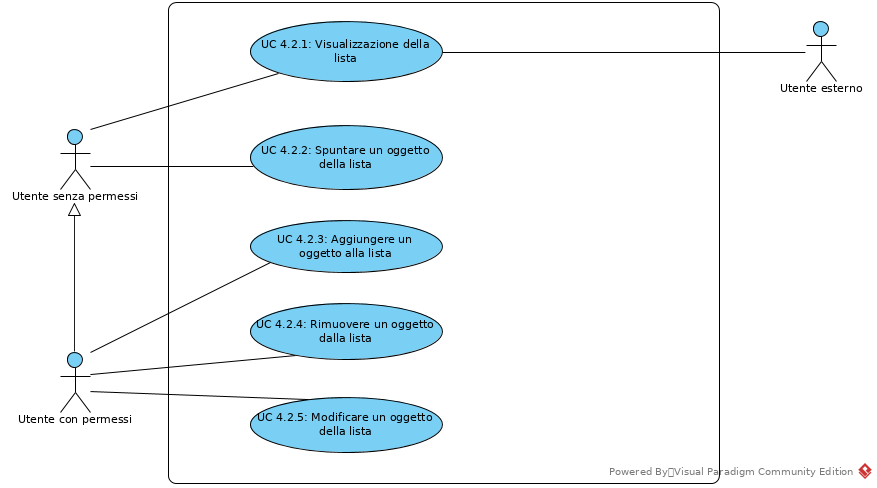
\includegraphics[scale=0.60]{Usecases/img/UC4.2.png}
	\caption{Caso d'uso UC 4.2: Interazione con la bolla lista-spesa.}
\end{figure}

\FloatBarrier
\begin{itemize}
\item \textbf{Attori:} Utente senza permessi, Utente con permessi, Utente esterno.
\item \textbf{Descrizione:} L'utente vuole interagire con la bolla lista-spesa e in base al tipo di utente potrà eseguire diverse azioni tra cui:
\begin{itemize}
\item Visualizzare la lista.
\item Spuntare un oggetto della lista.
\item Aggiungere un oggetto alla lista.
\item Rimuovere un oggetto dalla lista.
\item Modificare un oggetto della lista.
\end{itemize}
\item \textbf{Precondizione:} L'utente vuole interagire con la bolla lista-spesa. 
\item \textbf{Postcondizione:} L'utente ha interagito con la bolla lista-spesa con le modalità che la tipologia d'utente di cui fa parte permette.
\item \textbf{Scenario principale:}
	\begin{itemize}
	\item{Visualizzazione della lista (UC 4.2.1).}
	\item{Spunta di un oggetto della lista (UC 4.2.2).}
	\item{Aggiunta di un oggetto alla lista (UC 4.2.3).}
	\item{Rimozione di un oggetto dalla lista (UC 4.2.4).}
	\item{Richiesta di aiuto all'utilizzo della bolla lista spesa (UC 4.2.5).}
	\end{itemize}
\end{itemize}